\section{Functional Decomposition}

\subsection{Level 0 --- System Overview}
\begin{figure}[H]
\centering
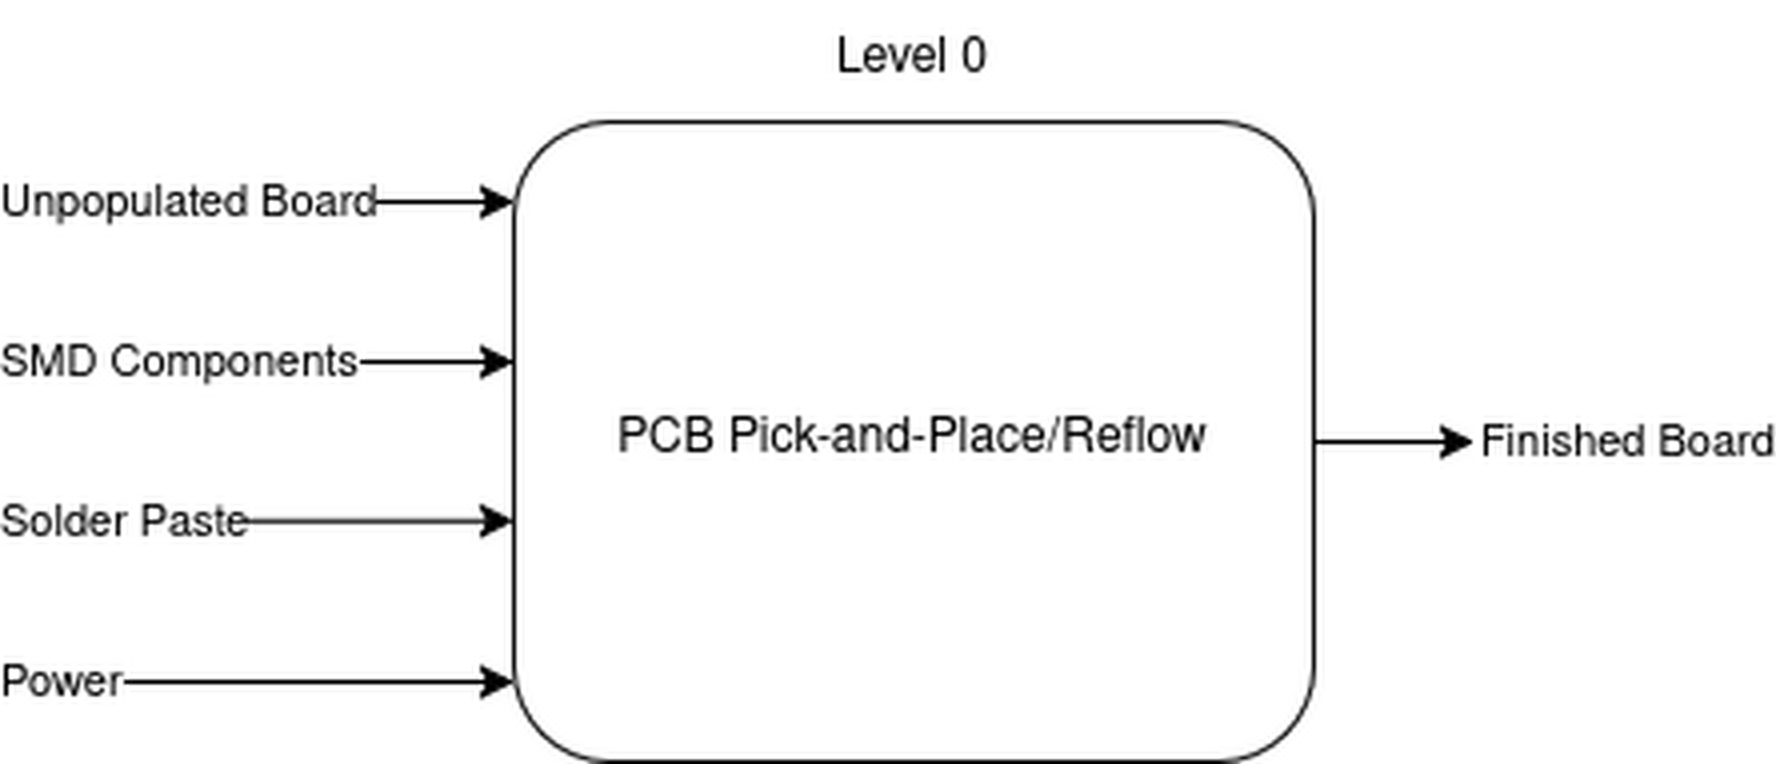
\includegraphics[width=0.7\textwidth]{Level0.png}
\caption{Level 0 Decompositon}
\label{fig:level0}
\end{figure}

\subsection{Level 1 Decomposition}
\begin{figure}[H]
\centering
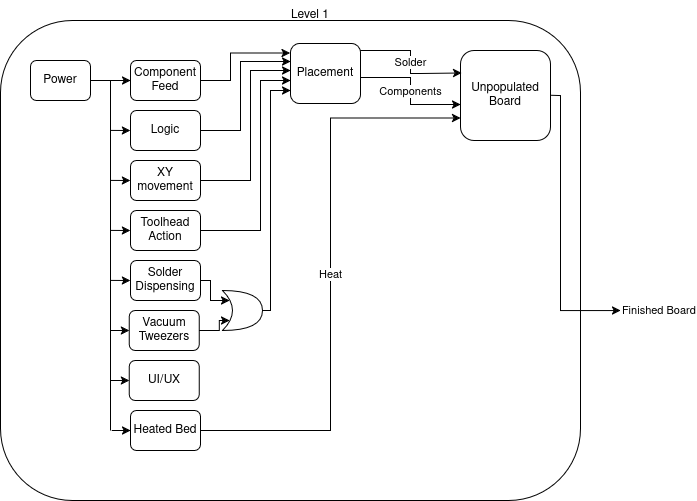
\includegraphics[width=\textwidth]{Level_1.png}
\caption{Level 1 Decomposition}
\label{fig:level1}
\end{figure}

\subsection{Level 2 --- Power}
\begin{figure}[H]
\centering
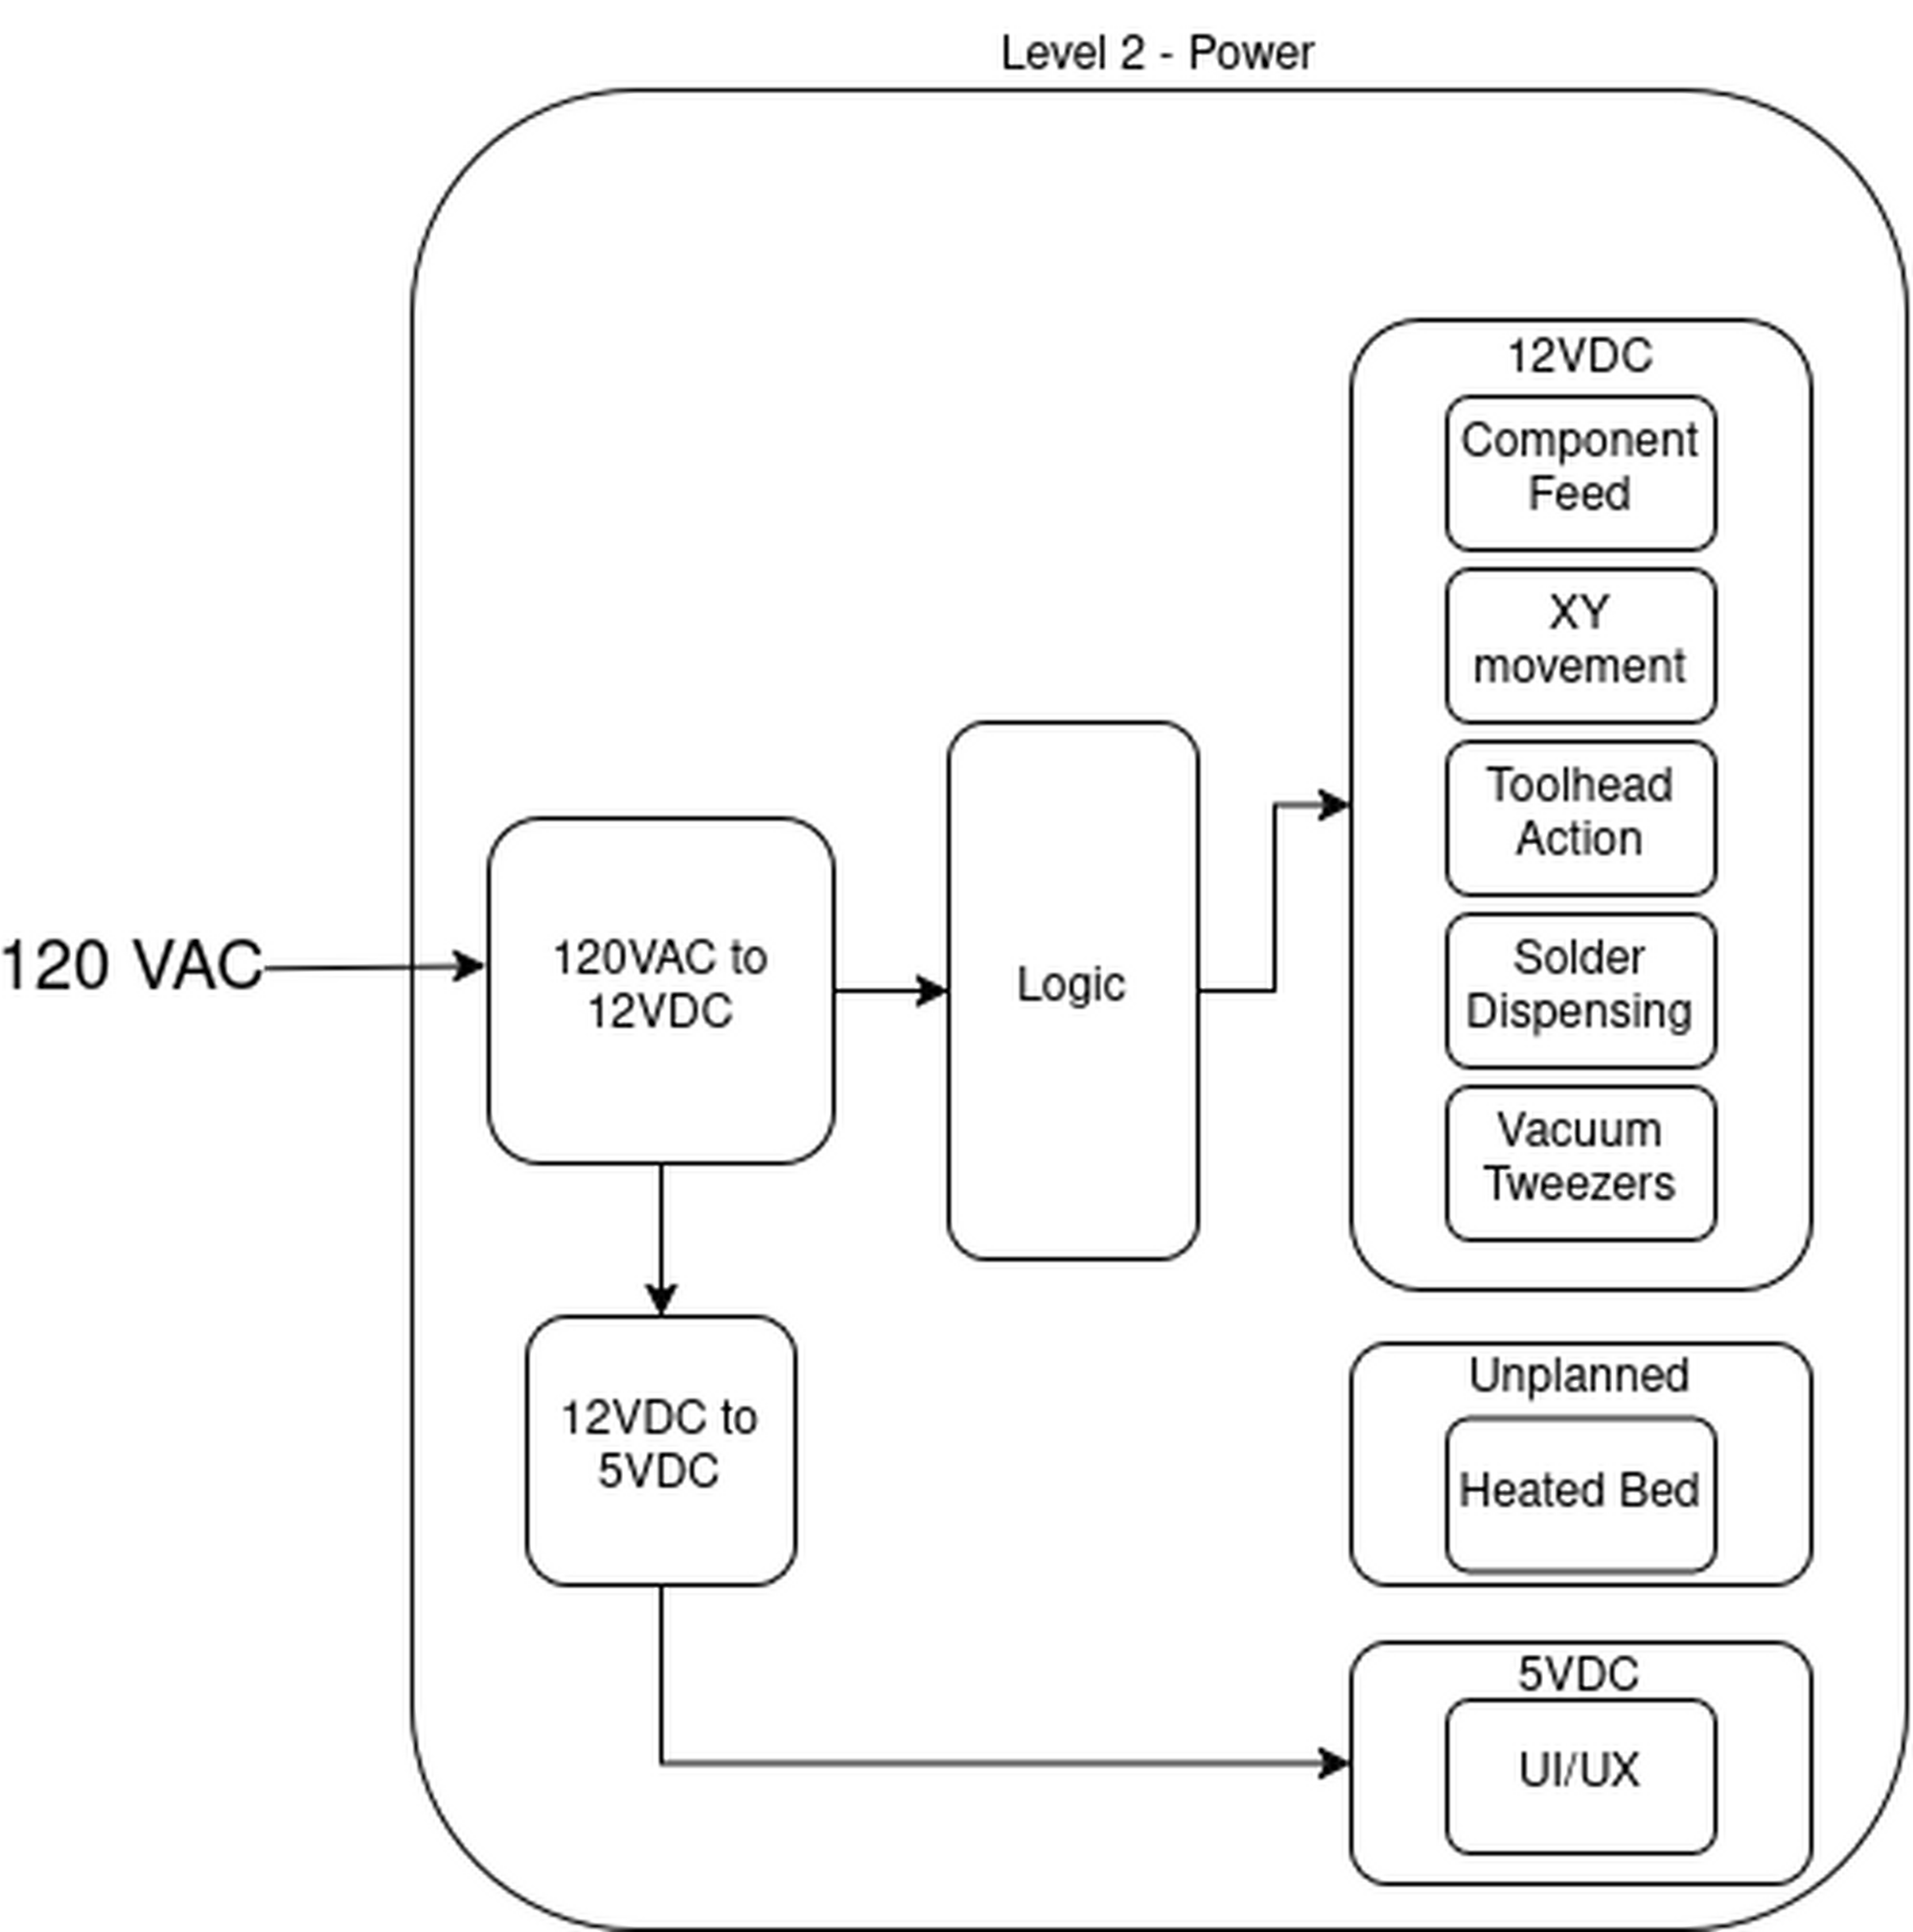
\includegraphics[width=0.85\textwidth]{Level2_power.png}
\caption{Level 2 Decomposition - Power}
\label{fig:level2_power}
\end{figure}

\subsection{Level 2 --- Logic \& UI/UX}
\begin{figure}[H]
\centering
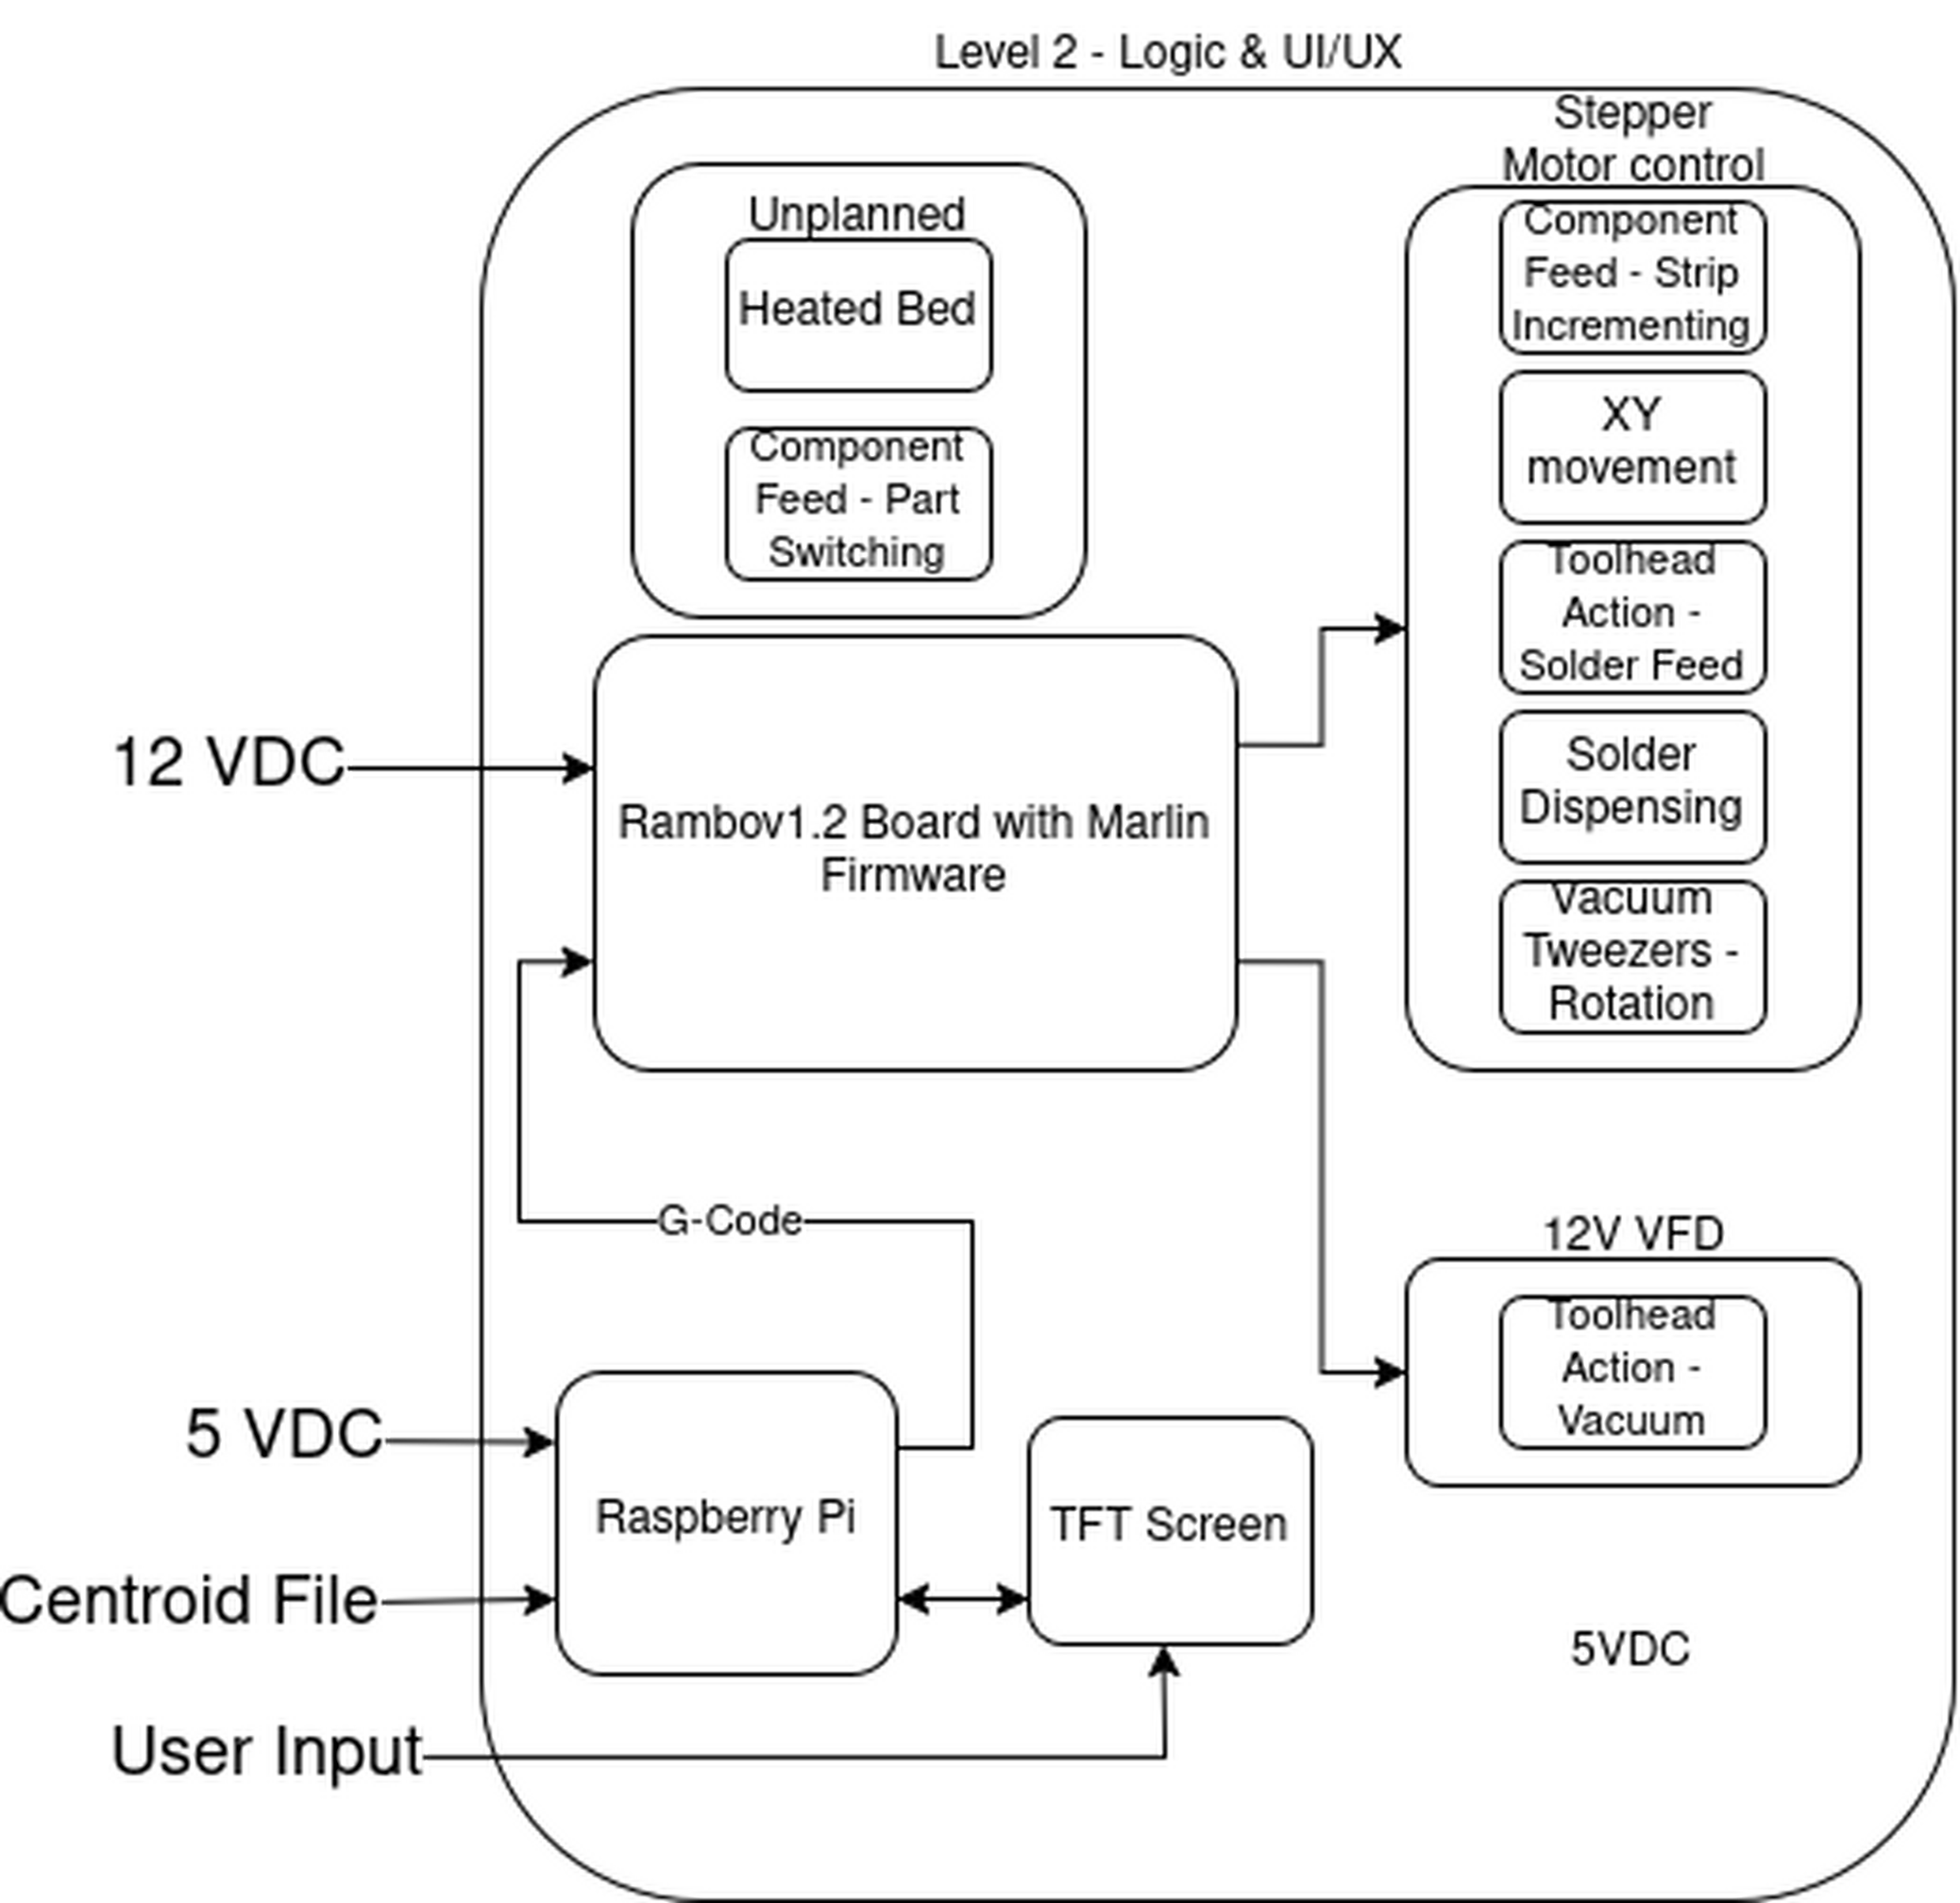
\includegraphics[width=\textwidth]{Level2_logic_ui_ux.png}
\caption{Level 2 Decomposition - Logic and UI/UX}
\label{fig:level2_logic}
\end{figure}

\subsection{Level 2 --- XY Movement}
\begin{figure}[H]
\centering
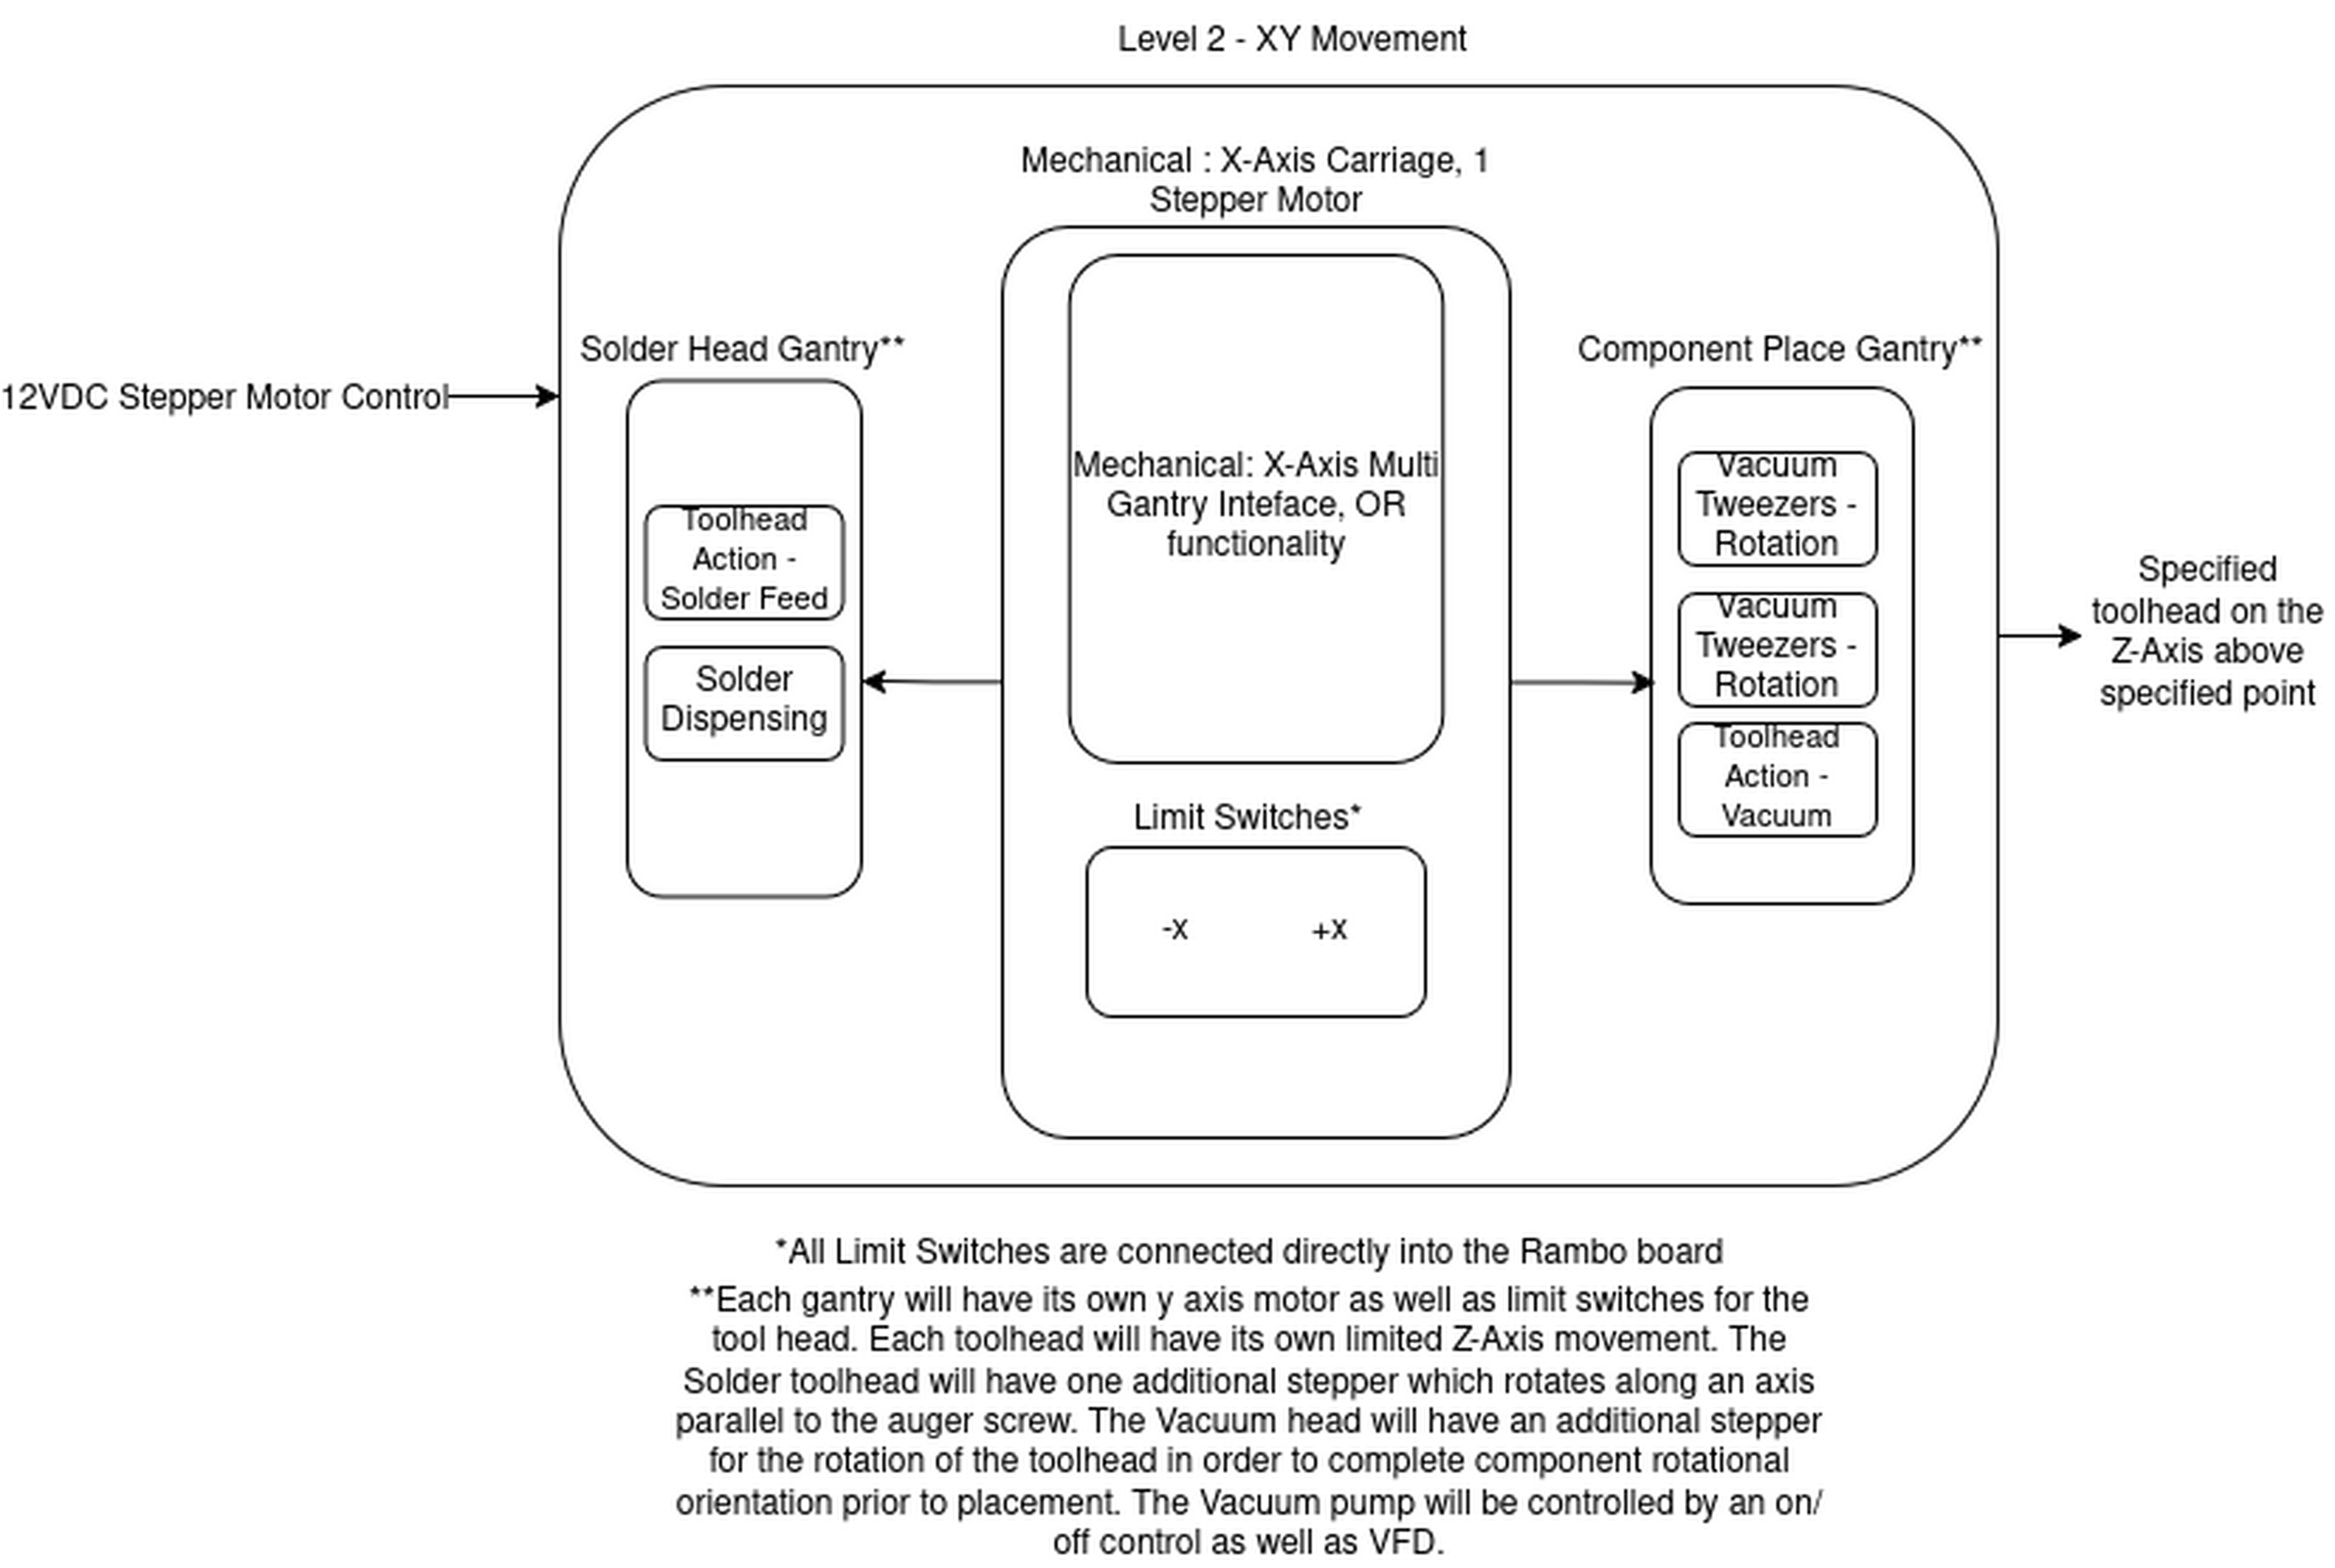
\includegraphics[width=\textwidth]{Level2_xy_movement.png}
\caption{Level 2 Decomposition of the XY Movement}
\label{fig:level2_xy}
\end{figure}

